\chapter{埃林厄姆图与冶金}\label{ch:b2:ellingham}

高炉以焦炭和热空气把红色岩石炼成液态铁，
日产量可达数千吨。这种炉子永远无法炼出铝、镁或钛，
尽管碳对它们同样便宜。
大多数金属以氧化物的形式存在于地下，冶炼金属即是
夺去其中的氧：哪种还原剂能做到，以及在何种温度下做到，
取决于标准吉布斯自由能。1944 年，哈罗德·埃林厄姆
把它们全部画在同一张图上，以温度为横坐标，各以 1 摩尔氧气为基准。
这张图一眼即可看出哪种金属能还原哪种氧化物，
为何高温下碳占优势，以及为何某些金属必须用
电解法制取。

\begin{recall}
\Cref{ch:b2:reaction-free-energy}：$\Delta_r G^\circ = \Delta_r H^\circ -
T\Delta_r S^\circ$，以及埃林厄姆近似（对 $T$ 呈直线，相变除外）。
\Cref{ch:b2:equilibrium-shifts}：$K^\circ$ 可由 $\Delta_r G^\circ$ 求出，并给出自由度，
以及某相消失时平衡的终止。
本科一年级分册：氧化数、氧化还原电对、碱性与酸性氧化物。
第 1 册：矿石。
\end{recall}

\begin{omfigure}
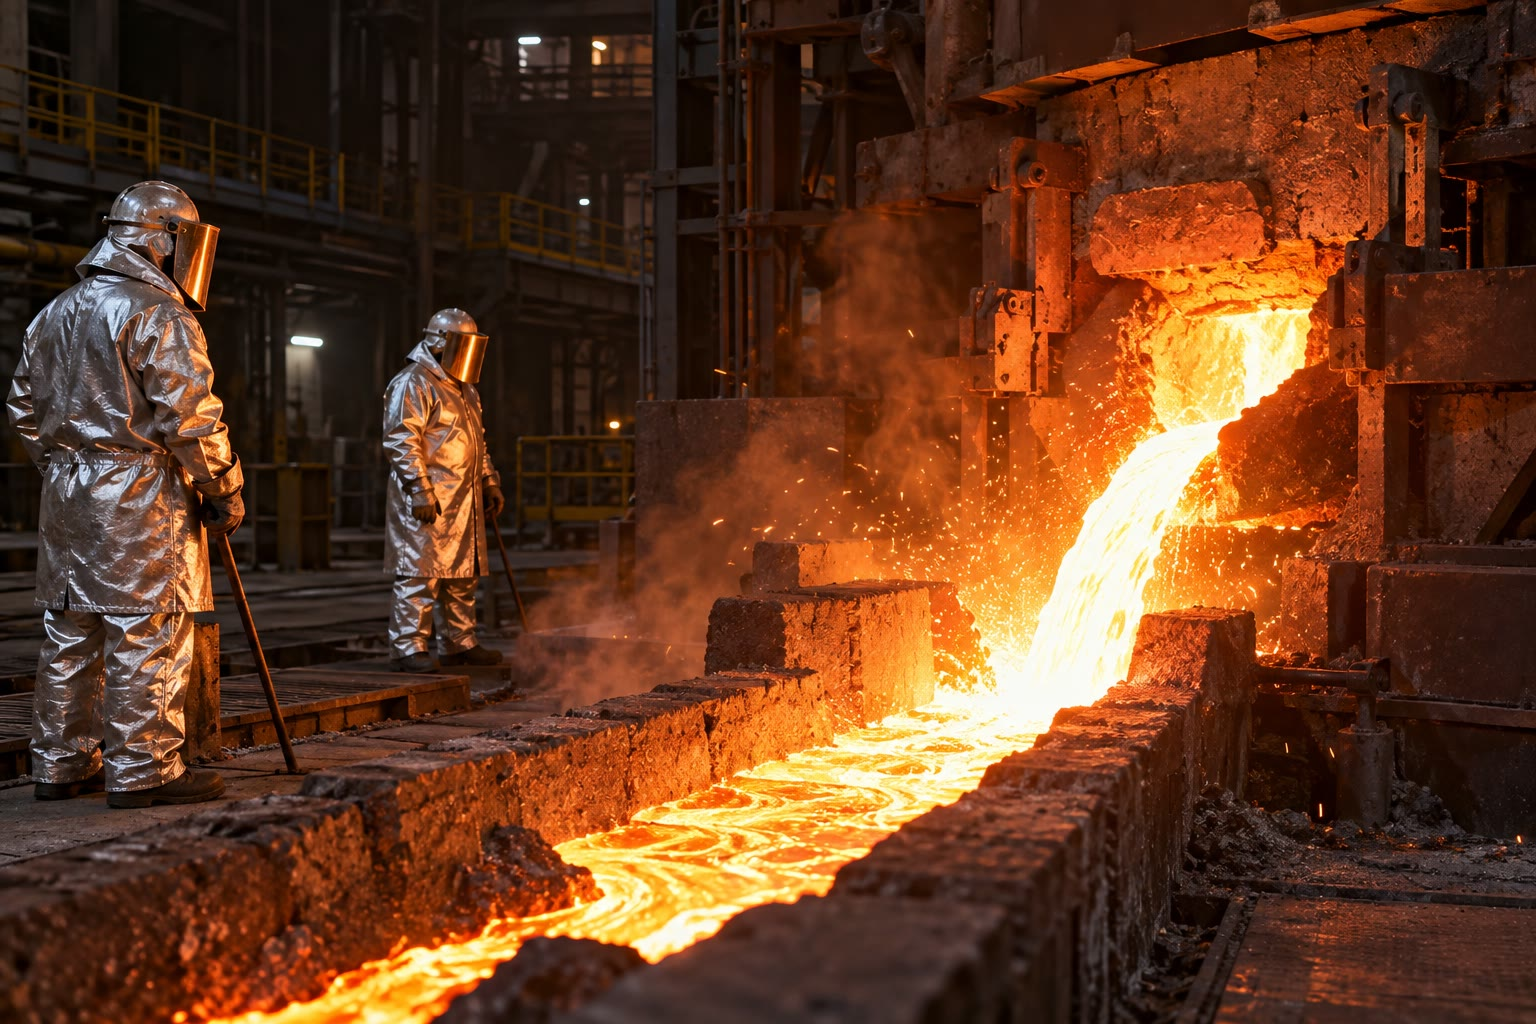
\includegraphics[width=0.62\linewidth]{images/book3/ai/b2-06-blast-furnace.jpg}

{\small 出铁：液态铁沿耐火通道流出，
旁有身穿隔热服的工人观看。炉内的温度与气体，
正是使一氧化碳能从
氧化铁中夺去氧的条件。}
\end{omfigure}

\section{埃林厄姆图}

为比较不同金属对氧的亲和力，
各反应均写成消耗同量公共试剂的形式。

\begin{definition}[埃林厄姆图]\label{def:b2:ellingham:diagram}
某一族氧化物的\emph{埃林厄姆图}\index{埃林厄姆图}，是
以温度为横坐标、其生成反应的标准吉布斯自由能为纵坐标的图像，
其中各生成反应均按 1 摩尔氧气书写，
\[
  \tfrac{2x}{y}\,\mathrm M + \ce{O2} \longrightarrow \tfrac{2}{y}\,\mathrm{M}_x\mathrm O_y ,
  \qquad \Delta_r G^\circ(T) \ \text{每摩尔 } \ce{O2} .
\]
\end{definition}

例如 \ce{2Zn + O2 -> 2ZnO}、\ce{4/3Al + O2 -> 2/3Al2O3}、\ce{2C + O2 ->
2CO}。纵坐标单位为 \unit{kJ}（每摩尔 \ce{O2}），
对图中所示的金属，纵坐标始终为负。

\begin{proposition}[直线]\label{prop:b2:ellingham:line}
在埃林厄姆近似下，每条线均为直线，斜率为 $-\Delta_r
S^\circ$。对于金属及其氧化物（二者均为凝聚相），$\Delta_r S^\circ$
接近于所消耗的 1 摩尔氧气的熵的负值，约为
$-\qty{200}{J/(K.mol)}$：
各直线随温度上升，且斜率近乎相同。
\end{proposition}

\begin{proof}
$\Delta_r G^\circ = \Delta_r H^\circ - T\Delta_r S^\circ$，其中 $\Delta_r
H^\circ$、$\Delta_r S^\circ$ 为常数。固体的摩尔熵约为数十
\unit{J/(K.mol)}，在金属与氧化物之间基本相互抵消，而所消耗的 1 摩尔
气体，其熵为 $S^\circ(\ce{O2}) = \qty{205}{J/(K.mol)}$。以锌为例，
$2(43.65) - 2(41.63) - 205.15 = \qty{-201.1}{J/(K.mol)}$。
% ledger: s0:ZnO_cr, s0:Zn_cr, s0:O2_g
\end{proof}

\begin{proposition}[直线的转折]\label{prop:b2:ellingham:break}
在金属熔化或沸腾的温度下，直线的斜率发生改变：
斜率增加 $\nu\,\Delta_{\text{trs}}S$，其中 $\nu$ 为反应中
金属的物质的量，$\Delta_{\text{trs}}S = \Delta_{\text{trs}}H/T_{\text{trs}}$。
氧化物发生相变时，斜率则相反地减小。
\end{proposition}

\begin{proof}
高于转变温度时，金属以其新相参与反应，新相的熵
比原相高出 $\Delta_{\text{trs}}S$：$\Delta_r S^\circ$ 减小 $\nu\,\Delta_{\text{trs}}S$，
斜率 $-\Delta_r S^\circ$ 也随之增加同样的量。$\Delta_r G^\circ$
本身是连续的，因为在 $T_{\text{trs}}$ 时两相的化学势相同。
对于氧化物，则符号相反。
\end{proof}

熔化使斜率稍有改变；沸腾使凝聚态的反应物变为气体，
则使斜率大为改变。锌在 \qty{1180}{K} 沸腾，高于此温度时，
生成氧化锌的反应每生成 2 摩尔氧化物便消耗 3 摩尔气体，
其直线陡然上升。镁在其
沸点以上同样如此。

\begin{omfigure}
\begin{tikzpicture}[lab/.style={anchor=west, font=\scriptsize, inner sep=1pt}]
\begin{axis}[omellingham,
  width=0.84\linewidth, height=11cm, xmin=300, xmax=2100, ymin=-1250, ymax=0,
  clip mode=individual,
  xlabel={$T$（K）}, ylabel={$\Delta_r G^\circ$（\unit{kJ} 每摩尔 \ce{O2}）},
  xtick={300,500,700,900,1100,1300,1500,1700,1900,2100},
  x tick label style={rotate=45, anchor=north east, font=\scriptsize}]
\addplot[black!60, thick] table[x=T, y=G] {figdata/out/bachelor-2-ellingham-a-HgO.dat};
\addplot[omProp, thick] table[x=T, y=G] {figdata/out/bachelor-2-ellingham-a-Cu2O.dat};
\addplot[omDef, thick] table[x=T, y=G] {figdata/out/bachelor-2-ellingham-a-FeO.dat};
\addplot[omExo, very thick] table[x=T, y=G] {figdata/out/bachelor-2-ellingham-a-ZnO.dat};
\addplot[black!60, thick] table[x=T, y=G] {figdata/out/bachelor-2-ellingham-a-Cr2O3.dat};
\addplot[omProp, thick] table[x=T, y=G] {figdata/out/bachelor-2-ellingham-a-TiO2.dat};
\addplot[omDef, thick] table[x=T, y=G] {figdata/out/bachelor-2-ellingham-a-Al2O3.dat};
\addplot[black!60, thick] table[x=T, y=G] {figdata/out/bachelor-2-ellingham-a-MgO.dat};
\addplot[omProp, thick] table[x=T, y=G] {figdata/out/bachelor-2-ellingham-a-CaO.dat};
\addplot[omThm, very thick] table[x=T, y=G] {figdata/out/bachelor-2-ellingham-a-C-CO.dat};
\addplot[omThm, thick, dashed] table[x=T, y=G] {figdata/out/bachelor-2-ellingham-a-C-CO2.dat};
\addplot[omThm, thick, dotted] table[x=T, y=G] {figdata/out/bachelor-2-ellingham-a-CO-CO2.dat};
\addplot[omDef, thick, dashed] table[x=T, y=G] {figdata/out/bachelor-2-ellingham-a-H2-H2O.dat};
% labels: inside for the two short lines, at the right end for the others
  \node[font=\scriptsize, black!70, anchor=south] at (axis cs:400,-60) {氧化汞 \ce{HgO}};
  \node[font=\scriptsize, omProp, anchor=south] at (axis cs:1100,-150) {氧化亚铜 \ce{Cu2O}};
\draw[omExo, thin] (axis cs:2100,-69) -- (axis cs:2150,-60) node[lab, text=omExo] {氧化锌 \ce{ZnO}};
\draw[omThm, thin] (axis cs:2100,-204) -- (axis cs:2150,-185) node[lab, text=omThm] {\ce{CO}/\ce{CO2}};
\draw[omDef, thin] (axis cs:2100,-259) -- (axis cs:2150,-235) node[lab, text=omDef] {\ce{H2}/\ce{H2O}};
\draw[omDef, thin] (axis cs:2100,-286) -- (axis cs:2150,-285) node[lab, text=omDef] {氧化亚铁 \ce{FeO}};
\draw[black!70, thin] (axis cs:2100,-393) -- (axis cs:2150,-365) node[lab, text=black!70] {氧化铬 \ce{Cr2O3}};
\draw[omThm, thin] (axis cs:2100,-396) -- (axis cs:2150,-415) node[lab, text=omThm] {\ce{C}/\ce{CO2}};
\draw[omProp, thin] (axis cs:2100,-567) -- (axis cs:2150,-540) node[lab, text=omProp] {二氧化钛 \ce{TiO2}};
\draw[omThm, thin] (axis cs:2100,-589) -- (axis cs:2150,-590) node[lab, text=omThm] {\ce{C}/\ce{CO}};
\draw[black!70, thin] (axis cs:2100,-600) -- (axis cs:2150,-640) node[lab, text=black!70] {氧化镁 \ce{MgO}};
\draw[omDef, thin] (axis cs:2100,-668) -- (axis cs:2150,-690) node[lab, text=omDef] {氧化铝 \ce{Al2O3}};
\draw[omProp, thin] (axis cs:2100,-765) -- (axis cs:2150,-765) node[lab, text=omProp] {氧化钙 \ce{CaO}};
\end{axis}
\end{tikzpicture}

{\small 埃林厄姆图：以每摩尔 \ce{O2} 计的氧化物标准生成
吉布斯自由能随温度的变化，数据由表列吉布斯自由能算得。
线越低，氧化物越稳定，对应金属的还原性越强。
每条金属线以其氧化物标注；\ce{C}/\ce{CO} 对应 \ce{2C + O2 -> 2CO}，
\ce{C}/\ce{CO2} 对应 \ce{C + O2 -> CO2}，\ce{CO}/\ce{CO2} 对应 \ce{2CO + O2 -> 2CO2}，
以及 \ce{H2}/\ce{H2O} 对应 \ce{2H2 + O2 -> 2H2O}，其中水为气态。}
% ledger: janafG:Cu2O.300, janafG:FeO.300, janafG:Cr2O3.300, janafG:TiO2.500, janafG:Al2O3.300, janafG:MgO.300, janafG:CaO.300, janafG:CO.300, janafG:CO2.300, janafG:H2O.300, dfh:ZnO_cr, dfh:HgO_cr, s0:HgO_cr, s0:Hg_l, s0:Hg_g, dfh:Hg_g (all temperatures in figdata/bachelor-2/ellingham.py)
\end{omfigure}

\section{读图}

\begin{definition}[平衡氧分压]\label{def:b2:ellingham:oxygen-pressure}
称某一金属–氧化物对在温度 $T$ 下的\emph{平衡氧分压}\index{平衡氧分压}，
即金属与氧化物共存于平衡时的氧气分压，
满足 $RT\ln(p_{\ce{O2}}/p^\circ) = \Delta_r
G^\circ(T)$，此处反应按每摩尔 \ce{O2} 书写。
\end{definition}

\begin{theorem}[金属与氧化物的区域]\label{thm:b2:ellingham:domains}
在氧分压为 $p_{\ce{O2}}$、温度为 $T$ 的气氛中，
金属被氧化的条件是 $RT\ln(p_{\ce{O2}}/p^\circ) > \Delta_r G^\circ(T)$，
氧化物被还原为金属的条件是 $RT\ln(p_{\ce{O2}}/p^\circ) < \Delta_r
G^\circ(T)$。在图上，氧化物稳定于其线之上，
金属位于其线之下。
\end{theorem}

\begin{proof}
金属与氧化物均为凝聚相且活度为 1，则 $Q = p^\circ/p_{\ce{O2}}$，且
$\Delta_r G = \Delta_r G^\circ + RT\ln Q = \Delta_r G^\circ - RT\ln(p_{\ce{O2}}/
p^\circ)$。当 $\Delta_r G < 0$ 时，氧化反应正向进行。
\end{proof}

在空气中（$p_{\ce{O2}} = \qty{0.21}{bar}$，$RT\ln 0.21$ 在室温时为 \qty{-4}{kJ/mol}，
在 \qty{1000}{K} 时为 \qty{-13}{kJ/mol}，
在本图的尺度上几乎为零），图中线位于横轴以下的各种金属
都会被氧化：室温下全部如此，甚至包括铜。
只有靠近顶部的氧化物（银、汞）在
适度加热下才会分解。

\begin{example}[汞的氧化物]\label{ex:b2:ellingham:hgo}
对于 \ce{2Hg + O2 -> 2HgO}，由 CODATA 推荐值可得 $\Delta_r H^\circ =
\qty{-181.6}{kJ/mol}$（液态汞）；高于汞的沸点时，
汞为气态，$\Delta_r H^\circ = \qty{-304.3}{kJ/mol}$，$\Delta_r
S^\circ = \qty{-414.6}{J/(K.mol)}$。该线在
$T = 304.3/0.4146 \approx \qty{734}{K}$ 处与零线相交：在空气中加热至该温度以上，
或在 \qty{1}{bar} 氧气中，红色氧化汞放出其中的氧——
这正是 1774 年氧气首次被分离出来的方式。
% ledger: dfh:HgO_cr, s0:HgO_cr, s0:Hg_l, s0:Hg_g, dfh:Hg_g, s0:O2_g (computed in figdata/bachelor-2/ellingham.py)
\end{example}

\begin{proposition}[何种金属还原何种氧化物]\label{prop:b2:ellingham:reduction}
在给定温度、标准条件下，金属 M 能还原金属 N 的氧化物，
当 M 的线位于 N 的线之下时成立。
还原反应的标准反应吉布斯自由能（按每摩尔转移的 \ce{O2} 计）
等于两线纵坐标之差。
\end{proposition}

\begin{proof}
还原反应等于 M 的氧化物的生成反应减去 N 的氧化物的生成反应，两者均
以每摩尔 \ce{O2} 计：$\Delta_r G^\circ = \Delta_r G^\circ_{\mathrm M} - \Delta_r
G^\circ_{\mathrm N}$，当 M 的线较低时该值为负。
\end{proof}

\begin{method}[读埃林厄姆图]\label{met:b2:ellingham:read-ellingham}
\begin{enumerate}
  \item 找出所考虑温度下的两条线。较低的那条线
        对应的氧化物更稳定，其金属可还原另一种氧化物。
  \item 竖直间距即每摩尔 \ce{O2} 计的 $\Delta_r G^\circ$：若间距为
        \qty{100}{kJ} 或更大，则表示还原实际上已完全。
  \item 两线相交处，还原的方向发生改变：
        读取相交时的温度。
  \item 注意其间断：若金属在该温度区间内沸腾，则以
        蒸气逸出，可蒸馏分离——或在冷却时再次被氧化。
\end{enumerate}
\end{method}

\begin{definition}[铝热还原]\label{def:b2:ellingham:aluminothermy}
称\emph{铝热还原}\index{铝热还原}为用铝粉还原金属氧化物的反应，
对所有线位于氧化铝线之上的氧化物均可进行，
且放热剧烈，以致混合物熔化：
\ce{Fe2O3 + 2Al -> Al2O3 + 2Fe}（铝热剂）用于焊接钢轨；\ce{Cr2O3 + 2Al ->
Al2O3 + 2Cr} 可制得无碳的铬。
\end{definition}

\begin{omfigure}
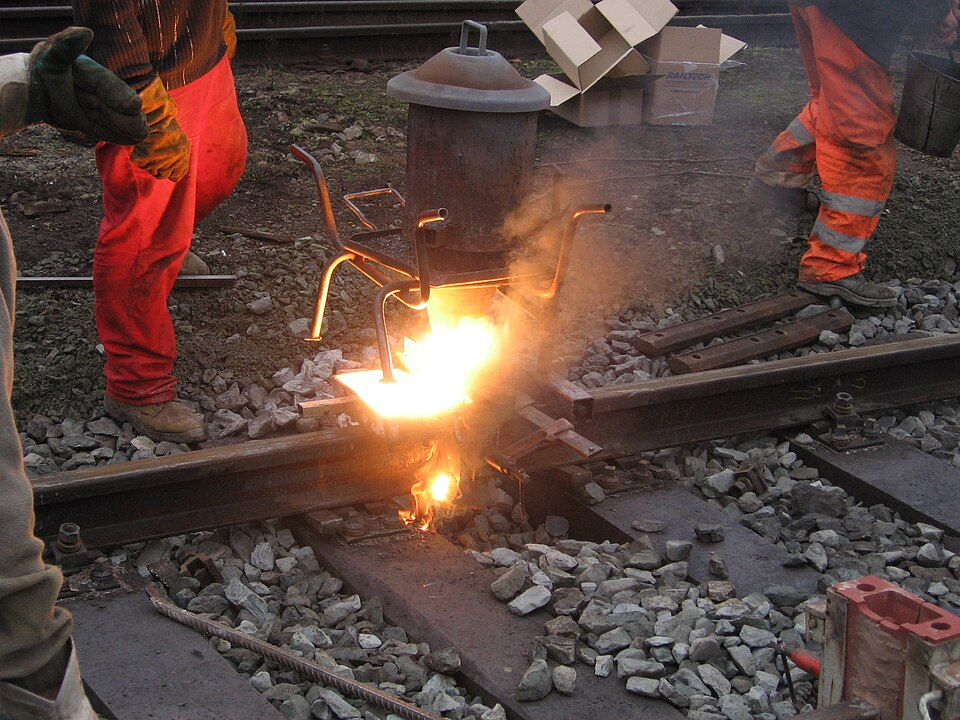
\includegraphics[width=0.5\linewidth]{images/book3/thermite.jpg}

{\small 钢轨的铝热焊接：氧化铁与铝在接头上方的坩埚中反应，
生成液态铁，液态铁流入两钢轨端之间的
铸型中。（照片：PetrS.，CC BY-SA 3.0，维基共享资源。）
}
\end{omfigure}

\section{碳与一氧化碳}

涉及碳的线有三条：
\begin{itemize}
  \item \ce{C + O2 -> CO2}：一摩尔气体生成一摩尔气体，$\Delta_r S^\circ
        \approx 0$，近乎水平的线，位于 \qty{-395}{kJ} 附近；
  \item \ce{2C + O2 -> 2CO}：一摩尔气体生成两摩尔气体，$\Delta_r S^\circ
        \approx \qty{+180}{J/(K.mol)}$，一条随温度\emph{下降}的线；
  \item \ce{2CO + O2 -> 2CO2}：三摩尔气体生成两摩尔气体，一条上升的线。
\end{itemize}

\begin{proposition}[高温下碳几乎可还原一切]\label{prop:b2:ellingham:carbon}
\ce{2C + O2 -> 2CO} 的线随温度升高而下降，并与
大多数金属氧化物的线相交：高于相交温度时，碳可还原
该氧化物，生成一氧化碳。氧化亚铁的相交温度约为
\qty{1040}{K}，氧化锌约为 \qty{1220}{K}；对于二氧化钛和氧化镁，其
相交温度约在 \qty{2000}{K} 附近或更高；氧化铝的更高，此时金属
与碳化合生成碳化物，或在气体冷却时再次被氧化。
\end{proposition}

\begin{proof}
碳线的斜率 $-\Delta_r S^\circ$ 为负（$\Delta\nu_{\text{g}}
= +1$），氧化物的线斜率为正：二者恰相交一次。温度
由计算所得的直线读出。
% ledger: janafG:CO.900, janafG:CO.1100, janafG:FeO.900, janafG:FeO.1100 (crossings computed in figdata/bachelor-2/ellingham.py)
\end{proof}

\begin{definition}[布杜阿尔平衡]\label{def:b2:ellingham:boudouard}
\emph{布杜阿尔平衡}\index{布杜阿尔平衡}为 \ce{C(s) + CO2(g) <=> 2CO(g)}，
为吸热反应，发生于碳与碳的两种氧化物之间。
\end{definition}

\begin{proposition}[碳上方气体的组成]\label{prop:b2:ellingham:boudouard}
体系碳 + \ce{CO} + \ce{CO2} 的自由度为 2：在给定的 $T$ 与总
压强 $p$ 下，一氧化碳的摩尔分数 $x$ 由 $x^2/(1 - x)
= K^\circ(T)\,p^\circ/p$ 确定。在 \qty{1}{bar} 下，
低于 \qty{700}{K} 时，气体几乎纯为 \ce{CO2}，高于 \qty{1200}{K} 时几乎纯为 \ce{CO}；三条碳线的
交点约在 \qty{975}{K}，此处 $K^\circ = 1$。
\end{proposition}

\begin{proof}
三种物种，一个反应，两相：$v = 3 - 1 + 2 - 2 = 2$。取 $p_{\ce{CO}}
= xp$，$p_{\ce{CO2}} = (1 - x)p$，则 $Q = x^2p/[(1 - x)p^\circ]$。当 $K^\circ = 1$ 时，
\ce{2C + O2 -> 2CO} 与 \ce{C + O2 -> CO2} 的标准吉布斯自由能
相等：两条线相交，第三条线亦然。
\end{proof}

\begin{omfigure}
\begin{tikzpicture}
\begin{axis}[
  width=0.62\linewidth, height=5.4cm, xmin=500, xmax=1500, ymin=0, ymax=1.05,
  axis x line=bottom, axis y line=left, xlabel={$T$ (K)},
  xtick={500,700,900,1100,1300,1500}, ytick={0,0.5,1},
  ylabel={\ce{CO} 的摩尔分数}, tick label style={font=\small},
  label style={font=\small}, clip=false]
\addplot[omThm, very thick] table[x=T, y=xCO] {figdata/out/bachelor-2-ellingham-b.dat};
\node[font=\scriptsize, anchor=west] at (axis cs:1150,0.55) {\ce{CO} 稳定};
\node[font=\scriptsize, anchor=west] at (axis cs:510,0.6) {\ce{CO2}（及碳）稳定};
\end{axis}
\end{tikzpicture}

{\small \qty{1}{bar} 下的布杜阿尔平衡：与碳处于平衡的气体中
一氧化碳的摩尔分数。}
% ledger: janafG:CO.700, janafG:CO2.700, janafG:CO.1100, janafG:CO2.1100 (computed in figdata/bachelor-2/ellingham.py)
\end{omfigure}

\section{高炉}

铁矿石（赤铁矿 \ce{Fe2O3}、磁铁矿 \ce{Fe3O4}）、焦炭和石灰石
从高炉顶部加入；热空气从
底部附近吹入。固体向下运动，与上升的热气体相遇，气体
在顶部离开，已被冷却。
\begin{itemize}
  \item 在风口处，焦炭在热空气中燃烧：\ce{C + O2 -> CO2}，而在
        其上方，碳过量时发生 \ce{CO2 + C -> 2CO}（布杜阿尔反应）：上升的
        气体主要是一氧化碳和氮气。
  \item 在上部，一氧化碳逐步还原铁的氧化物，
        \ce{3Fe2O3 + CO -> 2Fe3O4 + CO2}，\ce{Fe3O4 + CO -> 3FeO + CO2}，
        \ce{FeO + CO -> Fe + CO2}。前两步较易进行；对于最后一步，
        \ce{CO}/\ce{CO2} 的线略\textit{高于} \ce{FeO} 的线：其标准反应吉布斯自由能
        略为正，
        （$K^\circ \approx 0.3$，在 \qty{900}{K} 时），还原需要气体中
        \ce{CO} 的含量至少为 \ce{CO2} 的三倍，而这一条件由
        下方高温区的布杜阿尔平衡提供。
  \item 下部温度更高，碳本身还原剩余的氧化物，\ce{FeO + C ->
        Fe + CO}；铁溶解碳并熔化，
        与由石灰和矿石中二氧化硅形成的熔渣一同聚集于底部。
\end{itemize}

\begin{omfigure}
\begin{tikzpicture}[font=\small, >={Stealth}]
  \fill[gray!12] (-1.4,0) -- (-2.0,3.0) -- (-1.3,7.0) -- (1.3,7.0) -- (2.0,3.0) -- (1.4,0) -- cycle;
  \draw[thick] (-1.4,0) -- (-2.0,3.0) -- (-1.3,7.0) (1.4,0) -- (2.0,3.0) -- (1.3,7.0);
  \draw[thick] (-1.4,0) -- (1.4,0);
  \fill[orange!70!red] (-1.4,0) rectangle (1.4,0.35);
  \fill[yellow!50!orange] (-1.45,0.35) rectangle (1.45,0.6);
  \node[font=\scriptsize] at (0,0.17) {铁液};
  \node[font=\scriptsize] at (0,0.48) {熔渣};
  % tuyeres
  \draw[->, thick, omDef] (-3.2,1.2) -- (-1.75,1.2) node[pos=0, left] {热空气};
  \draw[->, thick, omDef] (3.2,1.2) -- (1.75,1.2);
  % charge and gas
  \draw[->, thick] (-0.6,7.9) -- (-0.6,7.1) node[pos=0, above left, xshift=6pt] {矿石、焦炭、石灰石};
  \draw[->, thick, omThm] (0.7,7.1) -- (0.7,7.9) node[pos=1, above right, xshift=-6pt] {炉顶气体（\ce{CO}、\ce{CO2}、\ce{N2}）};
  \draw[->, omThm, thick] (0.6,1.6) -- (0.6,6.4);
  \draw[->, thick] (-0.6,6.4) -- (-0.6,1.6);
  \node[omThm, font=\scriptsize, rotate=90] at (0.9,4.0) {气体上升};
  \node[font=\scriptsize, rotate=90] at (-0.9,4.0) {固体下降};
  % zones
  \node[anchor=west, align=left, font=\scriptsize] at (2.3,6.0) {\ce{3Fe2O3 + CO -> 2Fe3O4 + CO2}\\ \ce{Fe3O4 + CO -> 3FeO + CO2}};
  \node[anchor=west, align=left, font=\scriptsize] at (2.3,4.2) {\ce{FeO + CO -> Fe + CO2}};
  \node[anchor=west, align=left, font=\scriptsize] at (2.3,2.7) {\ce{CO2 + C -> 2CO}\\ \ce{FeO + C -> Fe + CO}};
  \node[anchor=west, align=left, font=\scriptsize] at (2.3,1.6) {\ce{C + O2 -> CO2}};
  \draw[densely dotted] (1.95,6.0) -- (2.3,6.0) (1.9,4.2) -- (2.3,4.2) (2.0,2.8) -- (2.3,2.8);
  \node[anchor=east, align=right, font=\scriptsize, black!60] at (-2.2,6.0) {较冷};
  \node[anchor=east, align=right, font=\scriptsize, black!60] at (-2.2,2.3) {较热};
  \draw[->, black!50] (-2.6,5.6) -- (-2.6,2.7);
\end{tikzpicture}

{\small 作为逆流反应器的高炉。固体向下，热的
还原性气体向上；铁的氧化物在上部较冷处
被一氧化碳还原，在下部较热处被碳还原。铁与
熔渣从底部放出。}
\end{omfigure}

\begin{omfigure}
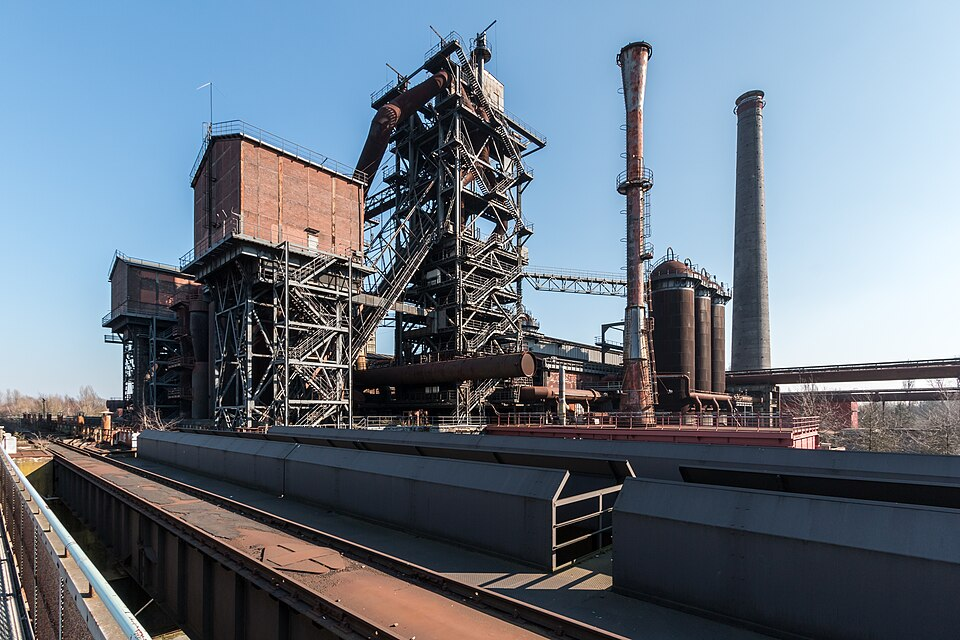
\includegraphics[width=0.6\linewidth]{images/book3/blast-furnace.jpg}

{\small 作为纪念物保存的一座高炉（杜伊斯堡-北，于
1985 年停用）：高耸的炉身，环绕的热空气送风管，以及
顶部的煤气导出口。（图片：Dietmar Rabich，CC BY-SA 4.0，维基共享资源。）}
\end{omfigure}

\section{获取金属的其他途径}

\begin{definition}[火法冶金与湿法冶金]\label{def:b2:ellingham:metallurgy}
\emph{火法冶金}\index{火法冶金}在高温下，通过在炉中还原金属的氧化物来提取金属。
\emph{湿法冶金}\index{湿法冶金}则从水溶液中提取金属。
两者通常的步骤是
\emph{焙烧}\index{焙烧}（在空气中加热硫化矿，使其转化为
氧化物，\ce{2ZnS + 3O2 -> 2ZnO + 2SO2}），\emph{浸出}\index{浸出}
（使金属的化合物溶解，常用硫酸，\ce{ZnO + 2H+ ->
Zn^2+ + H2O}），溶液的净化，例如通过
\emph{置换沉淀}\index{置换沉淀}（较不活泼金属的离子被
较活泼金属的粉末还原，\ce{Cu^2+ + Zn -> Cu + Zn^2+}），以及
金属的回收，常用电解法。
\end{definition}

图示说明了冶炼方法的分工。铁、锌、铅、锡都由
炉中的碳还原获得。铝的直线在任何可行温度下都远低于碳的直线，
故铝需用其熔融氧化物电解制得
（见\cref{ch:b2:batteries-electrolysis}）；镁可用电解法，或
在真空下用硅还原，此过程可移除镁蒸气；
钛则先将氧化物转化为氯化物，\ce{TiO2 + 2Cl2 + C -> TiCl4 +
CO2}（见\cref{exo:b2:reaction-free-energy:12}），再用镁还原氯化物
（即克劳尔法）。世界上大部分锌通过焙烧、
浸出和电解制得。湿法冶金路线可得到较纯的金属，
并避免处理锌蒸气。

\begin{omfigure}
\begin{tikzpicture}[font=\small, >={Stealth}, box/.style={draw, thick, rounded corners=2pt, align=center, minimum height=0.9cm, fill=white, text width=2.3cm}]
  \node[box] (r) at (0,0) {焙烧 \\ \ce{ZnS} $\to$ \ce{ZnO}};
  \node[box] (l) at (3.2,0) {浸出 \\ 在 \ce{H2SO4} 中};
  \node[box] (c) at (6.4,0) {净化 \\ （置换沉淀）};
  \node[box] (e) at (9.6,0) {电解 \\ \ce{Zn^2+} $\to$ \ce{Zn}};
  \draw[->, thick] (r) -- (l); \draw[->, thick] (l) -- (c); \draw[->, thick] (c) -- (e);
  \draw[->, thick, black!60] (r.north) -- ++(0,0.7) node[above] {\ce{SO2} $\to$ 硫酸};
  \draw[->, thick, omThm] (e.south) -- ++(0,-0.6) -| (l.south) node[pos=0.25, below] {酸回送};
  \draw[->, thick] (e.east) -- ++(0.8,0) node[right] {锌};
\end{tikzpicture}

{\small 锌的湿法冶金路线。焙烧炉产生的二氧化硫
制成浸出所用的硫酸；在电解阳极再生的酸
被送回浸出工序。}
\end{omfigure}

\section{练习}

\begin{exercise}[$\star$]\label{exo:b2:ellingham:1}
写出以下各直线所表示的反应：氧化亚铜、氧化铝、
一氧化碳和二氧化碳，每种均以 1 摩尔 \ce{O2} 计。
\end{exercise}

\begin{exercise}[$\star$]\label{exo:b2:ellingham:2}
由 CODATA 基本数据（$\Delta_f H^\circ(\ce{ZnO}) = \qty{-350.46}{kJ/mol}$，
$S^\circ$：\ce{ZnO} 43.65，\ce{Zn} 41.63，\ce{O2} \qty{205.15}{J/(K.mol)}），
求固态锌参与反应 \ce{2Zn + O2 -> 2ZnO} 时的 $\Delta_r G^\circ(T)$。
\end{exercise}

\begin{exercise}[$\star$]\label{exo:b2:ellingham:3}
利用图示，列出在
\qty{1500}{K} 下能还原氧化铬(III)的金属，以及不能还原的金属。
\end{exercise}

\begin{exercise}[$\star$]\label{exo:b2:ellingham:4}
解释图中三条含碳直线斜率的正负。
\end{exercise}

\begin{exercise}[$\star\star$]\label{exo:b2:ellingham:5}
计算氧化汞(II)在 \qty{600}{K} 时的平衡氧分压
（液态汞，$\Delta_r H^\circ = \qty{-181.6}{kJ}$，$\Delta_r S^\circ =
\qty{-216.5}{J/K}$，均以每摩尔 \ce{O2} 计）。在该温度下，汞在
空气中会被氧化吗？
\end{exercise}

\begin{exercise}[$\star\star$]\label{exo:b2:ellingham:6}
求铝热反应 \ce{Fe2O3 +
2Al -> Al2O3 + 2Fe} 在 \qty{298}{K} 下的 $\Delta_r G^\circ$。已知 $\Delta_f G^\circ = \qty{-743.5}{kJ/mol}$，
对应 \ce{Fe2O3}；\qty{-1582.3}{kJ/mol} 对应 \ce{Al2O3}。并说明
为何该反应虽放能很强，在室温下却不会开始进行。
% ledger: janafG:Fe2O3.298, janafG:Al2O3.298
\end{exercise}

\begin{exercise}[$\star\star$]\label{exo:b2:ellingham:7}
在图上找出一个温度，高于该温度时，碳可将氧化铁(II)
还原为铁并生成一氧化碳，并写出该反应。
\end{exercise}

\begin{exercise}[$\star\star$]\label{exo:b2:ellingham:8}
在 \qty{1100}{K} 下，$\Delta_f G^\circ(\ce{CO}) = \qty{-209.1}{kJ/mol}$，且
$\Delta_f G^\circ(\ce{CO2}) = \qty{-396.0}{kJ/mol}$。求
布杜阿尔平衡的 $K^\circ$，以及碳上方一氧化碳的摩尔分数，
总压为 \qty{1}{bar} 时的值。该气体与烟灰或铁接触时，
冷却至 \qty{700}{K} 时会发生什么变化？
% ledger: janafG:CO.1100, janafG:CO2.1100
\end{exercise}

\begin{exercise}[$\star\star$]\label{exo:b2:ellingham:9}
氢气有时用于还原氧化钨。利用水的直线，
解释为何在高温下氢气比一氧化碳是更好的还原剂，
而在低温下则较差。
\end{exercise}

\begin{exercise}[$\star\star\star$]\label{exo:b2:ellingham:10}
氧化镁可以被硅还原，\ce{2MgO + Si -> SiO2 + 2Mg}，
尽管图中每一温度下，二氧化硅的直线都位于氧化镁直线之上，
在 \qty{1500}{K} 时，镁为气体，表中给出每摩尔
\ce{O2}，氧化镁为 \qty{-845.5}{kJ}，二氧化硅为 \qty{-643.7}{kJ}。
计算该还原反应的 $\Delta_r G^\circ$，再求镁蒸气的压强，
低于此值时反应正向进行。真空炉如何利用这一点？
% ledger: janafG:MgO.1500, janafG:SiO2.1500
\end{exercise}

\begin{exercise}[$\star\star\star$]\label{exo:b2:ellingham:11}
求平衡时体系 \ce{FeO(s)}、\ce{Fe(s)}、\ce{CO(g)}、
\ce{CO2(g)} 的自由度。对高炉上部
逸出的气体，这意味着什么？
\end{exercise}

\begin{exercise}[$\star\star\star$]\label{exo:b2:ellingham:12}
以铁屑进行置换沉淀，从铜的浸出液中提纯铜。
利用本科一年级分册中的标准电极电势（$E^\circ(\ce{Cu^2+}/\ce{Cu})
= \qty{0.34}{V}$，$E^\circ(\ce{Fe^2+}/\ce{Fe}) = \qty{-0.41}{V}$），
求反应 \ce{Cu^2+ + Fe -> Cu + Fe^2+} 的平衡常数，以及
当溶液中含 \qty{1.0}{mol/L} 的
\ce{Fe^2+} 时，铜离子的残留浓度。
\end{exercise}

\section{问题：火法炼锌}

\begin{problem}[{周末问题——氧化锌与一氧化碳的埃林厄姆线，
碳还原氧化锌的温度，炉子的自由度，
以及锌蒸气的液化}]
\label{pb:b2:ellingham:1}
电解法出现之前，锌是将其氧化物与碳
在黏土蒸馏罐中加热制得的。数据（CODATA，及锌的 JANAF 表）：$\Delta_f H^\circ(\ce{ZnO})
= \qty{-350.46}{kJ/mol}$；$S^\circ$（\unit{J/(K.mol)}）：\ce{ZnO} 43.65、\ce{Zn}
41.63、\ce{O2} 205.15；锌在 \qty{692.7}{K} 熔化（$\Delta_{\text{fus}}H =
\qty{7.32}{kJ/mol}$），在 \qty{1}{bar} 下于 \qty{1180.2}{K} 沸腾
（$\Delta_{\text{vap}}H = \qty{115.3}{kJ/mol}$）。对 \ce{2C + O2 -> 2CO}，
数据表给出 $\Delta_r G^\circ = \qty{-418.2}{kJ}$（\qty{1100}{K} 时）和
\qty{-453.0}{kJ}（\qty{1300}{K} 时）。
% ledger: dfh:ZnO_cr, s0:ZnO_cr, s0:Zn_cr, s0:O2_g, hT:Zn_cr.692, hT:Zn_l.692, hT:Zn_l.1180, hT:Zn_g.1180, dfh:Zn_g, janafG:CO.1100, janafG:CO.1300

\medskip
\noindent\textbf{第一部分——氧化锌的线。}
\begin{enumerate}
  \item 计算 $\Delta_r H^\circ$ 与 $\Delta_r S^\circ$，反应 \ce{2Zn(s) + O2 ->
        2ZnO} 在 \qty{298}{K} 时的值。
  \item 写出熔点以下的 $\Delta_r G^\circ(T)$。
  \item 计算锌的熔化熵与汽化熵。
  \item 写出熔点与沸点之间的 $\Delta_r G^\circ(T)$。
  \item 写出沸点以上的表达式。
  \item 计算三段直线的斜率，并说明为何最后一段陡得多。
  \item 验证三个表达式在转变温度处相互一致。
\end{enumerate}

\medskip
\noindent\textbf{第二部分——碳的线。}
\begin{enumerate}[resume]
  \item 由表中两个数值，写出 \ce{2C + O2 -> 2CO} 的直线
        在 \qty{1100}{K} 与 \qty{1300}{K} 之间写成 $a + bT$ 的形式。
  \item 推出其 $\Delta_r S^\circ$，并说明其符号的原因。
  \item 写出还原反应 \ce{ZnO + C -> Zn(g) + CO}，及其 $\Delta_r
        G^\circ(T)$，并将其表示为两直线之差（以每摩尔 \ce{O2} 计）。
  \item 求两直线相交处的温度。
  \item 为何该温度须高于
        锌的沸点？
\end{enumerate}

\medskip
\noindent\textbf{第三部分——蒸馏罐。}
\begin{enumerate}[resume]
  \item 求体系 \ce{ZnO(s)}、\ce{C(s)}、\ce{Zn(g)}、
        \ce{CO(g)} 的自由度，其中锌与一氧化碳仅由还原反应生成。
  \item 在 \qty{1}{bar} 下、\qty{1300}{K} 的蒸馏罐中，若反应进行完全，
        锌与一氧化碳的分压各为多少？
  \item 计算该还原反应在 \qty{1300}{K} 时的 $\Delta_r G^\circ$，以及
        相应的 $K^\circ$。
  \item 说明蒸馏罐为何应略高于两线交点
        的温度运行，而不宜远高于此温度。
\end{enumerate}

\medskip
\noindent\textbf{第四部分——冷凝器。}
\begin{enumerate}[resume]
  \item 将蒸气导入较冷的冷凝器，写出锌蒸气
        可被二氧化碳再氧化的反应。
  \item 利用图示说明，气体为何必须保持不含
        二氧化碳。
  \item 为何锌必须迅速液化，而非缓慢液化？
  \item 按所写的还原反应，计算每吨锌所需
        碳的质量。
  \item 计算该还原反应在约
        \qty{1300}{K} 下每吨锌吸收的热量（$\Delta_r H^\circ$ 取自
        第一、第二部分的表达式）。
  \item 说明在标准条件下，超过何温度时碳
        可还原氧化锌。
\end{enumerate}
\end{problem}
